\chapter{Background}
\label{chap:Background}

% NOTE: (aver) Explain important topics for the reader to understand

\section{Distributed Ledger Technology} % (fold)
\label{sec:Distributed Ledger Technology}

Distributed Ledger Technology, DLT, refers to the technology of the decentralized database, which provides control over
the development of data between various entities through a peer-2-peer network. It offers immutability, as the ledgers
are append-only, as well as distributed consensus mechanisms, controlling how and which data is added to the blockchain
and also replicate data to participating nodes. \cite{skarmeta-interledger-management-2020}

Validators..

Nodes..

Interledger Approaches..

% TODO: (aver) look for further definition and sources
\subsection{Blockchains} % (fold)
\label{sub:Blockchains}
As defined by \cite{diam-iot-2020} a blockchain is a distributed data structuring organizing a growing list of
transaction records into a chronologically linked sequence of data blocks, which is achieved by a decentralized
peer-2-peer network, consisting of a cluster of participating nodes. Blocks are continuously appended to the blockchain
through the \textit{mining} process, executed by distrustful peers. The mining process includes the verification of
broadcast transactions to specific nodes in the peer-2-peer network. Through a consensus mechanism the blocks are
conjoined to the blockchain. The result is a chain of blocks that ensures the integrity of existing blocks, leading to a
DLT without a need for a central authority.

There is a major distinction between \textit{permissioned} and \textit{permissionless} blockchains.
Everyone may join a permissionless blockchain, given in some cases they fulfill certain requirements, in contrast to
permissioned blockchains, where only approved members may join. \cite{hyperledger:aries-rfc} This requires a central
authority to fulfill this step, but given some environments, such as enterprise, it is necessary, see
Section~\ref{sec:Hyperledger Fabric}.

Permissioned networks boast improved performance over permissionless on on e.g., transaction verification, as only
approved members are in the network. To offset the absence of trust, in permissionless blockchains, typically mined
cryptocurrencies and or transaction fees. Therefore in permissioned the cost of using a fault-tolerant consensus
mechanism.

% TODO: (aver)
% - add further explanation and highlight difference to DLT
% - possibly explain privacy/confidentiality and PoW/PoC concepts
On that note a blockchain is a subset of the DLT. \cite{diam-iot-2020}
% subsection Blockchains (end)

\subsection{Smart Contract} % (fold)
\label{sec:Smart Contract}
% TODO: (aver) look for further definition and sources
Further defined by \cite{diam-iot-2020} a smart contract specifies a computer transaction protocol which is based on the
execution of terms of the contract upon fulfillment of some pre-conceived condition(s).
Relating back to blockchains, the smart contract is a part of some block, that is stored and verified there in the form
of code until execution. Its state consists of the contracts balance and an internal storage, that is updated on each
invocation of the contract. A user can send a transaction to the contract address, which triggers the state transition
of the contract and the data being written to the internal storage. A smart contract may perform a predefined logic and
also interact with other accounts by sending messages or transferring funds.

Most smart contracts apply the \textit{order-and-execute} architecture, in which the consensus protocol first validates
and orders transactions, then propagates it to its peer nodes and finally each peer executes the transaction
sequentially. The order-and-execute architecture requires deterministic execution, otherwise no consensus consensus can
be reached. To address non-determinism usually a Domain Specific Language, DSL, is used, such as \textit{Solidity}.
% subsection Smart Contract (end)

\subsection{Consensus Protocols} % (fold)
\label{sub:Consensus Protocols}
\textbf{\textit{TODO}}
CFT (crash fault-tolerant) or BFT (byzantine fault-tolerant)
% subsection Consensus Protocols (end)
% section Distributed Ledger Technology (end)

\section{Verifiable Credentials and Identity Management} % (fold)
\label{sec:Verifiable Credentials and Identity Management}

\subsection{Verified Credentials} % (fold)
\label{sub:Verified Credentials}
In contrast to identification through physical means, such as passports and driver licenses, the
\textit{Verifiable Credential, VC}, model tries to achieve similar portability, alas in a digital wallet, be it on a
phone or other edge device. \cite{w3c2019verifiablecredentials}

\textit{Digital Identity} is the digital reference to a person or subject \cite{Domingo_2020}, with which it/they in
response to requests for digital identification, authentication or proofs of authentication is presented. Also of
importance is that there is a unique identifier, that is connected to the digital identity.
\cite{Sedlmeir_Smethurst_Rieger_Fridgen_2021}
In general identities come with \textit{identifiers}, such as names, social security number, mobile number, date of
birth etc. \cite{eth-decentralized-identity}.

Support for verifiable credentials and digital wallets has been growing, e.g., in Canada \cite{preukschat2021self},
where Canada's Verifiable Organizations Network, VON, permits storage of credentials inside Hyperledger Aries
\cite{hyperledger:wiki}. VON allows the issuing of digital licenses, permits and registrations to legal entities using
VC.
The European Blockchain Services Infrastructure also uses VCs to issue documents from public institutions, such as
digital diplomas and social security passes. \cite{williams2020cross}

An example VC Document can be seen in Code Listing~\ref{code:vc-doc}.
% subsection Verified Credentials (end)

\subsection{Decentralized Identifiers} % (fold)
\label{sec:Decentralized Identifiers}
\textit{Decentralized Identifiers, DIDs}, not to be confused with Decentralized Identities, are often used by
decentralized identity protocols. \cite{w3c2022did} They are not issued by a centralized body and are stored on DLTs
or on peer-2-peer networks, which makes DIDs globally unique, resolvable with high quality and cryptographically
verifiable. \cite{w3c-did-primer} For example, an Ethereum account in itself is a valid DID and one can create as many
of them as one wishes. \cite{eth-decentralized-identity}.

According to \cite{eth-decentralized-identity} two main components make DIDs possible:
\begin{itemize}
	\item \textbf{Public Key Infrastructure (PKI)}: Using a public and private key for an entity, one can
	      authenticate user identities e.g., in a blockchain network such ash Ethereum and prove digital ownership
	      of assets.
	      The private key can decrypt and or signs, while the public key verifies or encodes.
	\item \textbf{Decentralized Datastores}: the blockchain as verifiable data registry is open, trustless and a
	      decentralized repository of information and through the existence of public blockchains the need to store
	      identifiers in centralized registries is eliminated.
\end{itemize}

Each DID is made up of three elements separated by colons as seen below \cite{w3c2022did}:
% \underbrace{\vphantom{\text{j}}\text{did}}_{\text{scheme}} :
\begin{align*}
	\underbrace{\text{did}}_{\text{Scheme}} :
	\underbrace{\text{method}}_{\text{Method}} :
	\underbrace{\text{1234567890abcdefg}}_{\text{Method-Specific Identifier}}
\end{align*}

The scheme is fixed to be DID, while the method summaries and describes how the DID works with a specific blockchain
and the specifications of DID deployment. Finally the method-specific identifier guarantees to be unique within the
context of the DID method.

A DID document can be of format JSON or JSON-LD, which is a JSON based format to represented linked data \cite{w3c2022did}.
An example can be seen in Code Listing~\ref{code:did-doc}. There are further optional identifiers and keys in such a
document explained in depth in the W3C specification \cite{w3c2022did}. Mainly it consists out of the identifiers, the
DID, which is required, a \textbf{controller} that may dispose over it and aliases through \textbf{alsoKnownAs}.
The next section entails \textbf{Verification Methods}, which may list multiple ways of verifying interactions with the
DID and other associated parties. The third Section \textbf{Verification Relationships} describes the relationship
between a DID and its verification method(s).
Finally the \textbf{Services} part describes what endpoints there are for the DID to interact or advertise, including
decentralized identity management services for further discovery, authentication, authorization, or interaction.

Although DIDs are integral to managing decentralized identities, they are not enough on their own, as they do not
provide meaningful identity attributes. In order to establish a trust-relationship between DID entities, the above
mentioned VCs prove useful. \cite{w3c2019verifiablecredentials}

\subsubsection{DIDComm} % (fold)
\label{sec:DIDComm}
\textbf{\textit{TODO}}
% subsubsection DIDComm (end)
% subsection Decentralized Identifiers (end)

% TODO: (aver) Either relate to this table from the paper, or port it into my thesis.
% \cite{Sedlmeir_Smethurst_Rieger_Fridgen_2021} summaries how centralized threats or problems in today's environment may
% be countered by decentralized solutions. ...
% \begin{table}
% 	\caption{Sedlmeir et al. (2021): Centralized problems and proposed decentralized solutions}
% 	\label{tab:Centralized problems and proposed decentralized solutions}
% 	\begin{center}
% 		\begin{tabular}[c]{|l|l|}
% 			\hline
% 			\textbf{Diagnosed Problems} & \textbf{Proposed Solutions} \\
% 			\hline
% 			Big-Tech and Government Surveillance & Non correlatable identifiers \\
% 			\hline
% 		\end{tabular}
% 	\end{center}
% \end{table}

% section Verifiable Credentials and Identity Management (end)

% TODO: (aver) explain Sovereignty
% \section{Sovereignty} % (fold)
% \label{sec:Sovereignty}
% Self-sovereign Identity, SSI, is compromised of 3 main pillar, blockchains, DIDs, and VCs.
% % section Sovereignty (end)


\section{Manufacture Usage Description} % (fold)
\label{sec:Manufacture Usage Description}

MUD has been developed by the International Engineering Task Force, IETF, with following goals and intents in mind:
\cite{rfc8520-mud}
\begin{itemize}
	\item Substantially reduce the threat surface on a device to those communications intended by the manufacturer.
	\item Provide a means to scale network policies to the ever-increasing number of types of devices in the network.
	\item Provide a means to address at least some vulnerabilities in a way that is faster than the time it might
	      take to update systems. This will be particularly true for systems that are no longer supported.
	\item Keep the cost of implementation of such a system to the bare minimum.
	\item Provide a means of extensibility for manufacturers to express other device capabilities or requirements.
\end{itemize}

MUD does not entail address network authorization of general purpose computers, it simply creates a suggestion than can
be followed.
The architecture of Devices using MUD can be seen in Figure~\ref{fig:NIST MUD Reference Architecture}, which is the
reference architecture by NIST \cite{dodson2021securing} but it can be found in similar fashion inside the RFC
specification.

\begin{figure}
	\begin{center}
		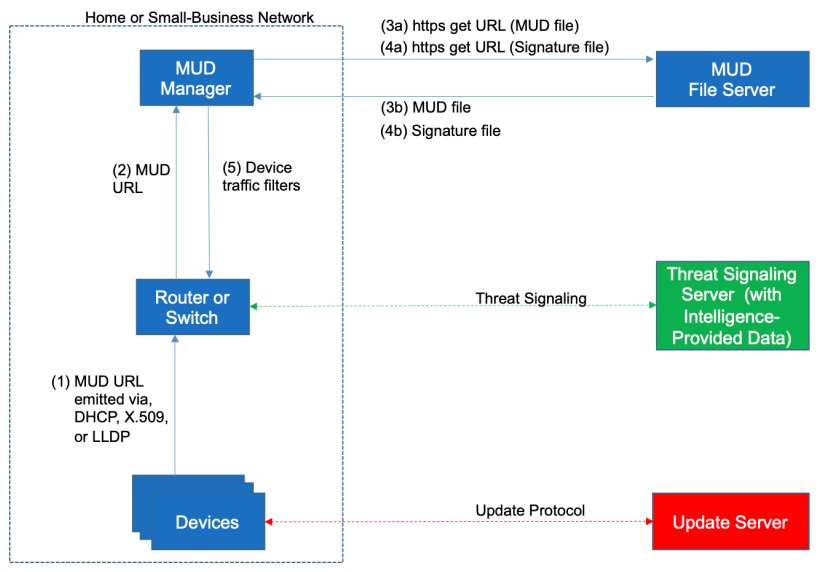
\includegraphics[width=0.95\textwidth]{figures/nist-mud-arch.png}
	\end{center}
	\caption{NIST MUD Reference Architecture}
	\label{fig:NIST MUD Reference Architecture}
\end{figure}
% section Manufacture Usage Description (end)

\section{Physical Unclonable Function} % (fold)
\label{sec:Physical Unclonable Function}

% TODO: (aver) add difference to 'physically unclonable function'

In order to be able to track IoT nodes in a blockchain, they need to be uniquely identifiable, in our case even in a
distributed manner, using e.g., Distributed Identifiers, DIDs.
Common practices are based on placing a cryptographic key into a nonvolatile electrically erasable programmable
read-only memory (EEPROM) or battery-backed static random-access memory (SRAM) and use hardware cryptographic operations
such as digital signatures or encryption, which is all expensive in design and power consumption. \cite{herder2014physical}

PUFs are unpredictable and uncontrollable, therefore making it unclonable and an ideal security vector. They are
dependent on random physical factors introduced during manufacturing, e.g., inequalities of SRAM cells, although factors
such as the altering of the physical components, voltage and temperature need to be taken into account. \cite{vinagrero2023sram}
For reasons of simplicity and because it is not the main focus of this thesis, we will neglect this aspect.
% TODO: Specify assumptions in another paragraph

By implementing the Challenge-Response Pair, CRP, is used to evaluate the microstructure, whereas a physical challenge
makes the device react, the response, in an unpredictable, but repeatable way.
In order to turn this 'silicon key' into a cryptographic root key, processing algorithms need to be applied, that ensure
that the distribution of 0s and 1s are uniform. \cite{herder2014physical}

\subsection{SRAM-Based PUF Readouts} % (fold)
\label{sec:SRAM-Based PUF Readouts}

Methods of creating identifiers that are unique to devices exist, such as SRAM-Based Physical Unclonable Function, PUF,
readouts. Therein PUFs are among the most cost-effective security primitives to establish hardware trust.
\cite{holcomb2007initial}

Even though the evaluation process of the characterization of guarantee over lifetime and differing operating conditions
are still subject to research following metrics have become widespread: \textit{reliability}, the variation of bit-wise
startup patterns; \textit{uniformity}, i.e., the repeatability and reproducibility on a given device after any amount of
restarts; \textit{uniqueness}, the probability of other devices with same signatures; \textit{bit-aliasing}, the
probability of specific bit position of the signature to be biased towards 0 or 1. \cite{vinagrero2023sram}
% subsection SRAM-Based PUF Readouts (end)

% TODO: (aver) challenges, vulnerabilities

% section Physical Unclonable Function (end)
\section{Over the Air IoT updating} % (fold)
\label{sec:Over the Air  IoT updating}
In order to stray away from the classic client-server architecture for updating devices, which demonstrate a single
point of failure, we will discuss other decentralized methods to achieve Over the Air, OTA, updates for IoT devices.

\subsection{Distributed OTA} % (fold)
\label{sub:Distributed OTA}
\textbf{\textit{TODO}}
% subsection Distributed OTA (end)
% section Over the Air IoT updating (end)

\section{Networking} % (fold)
\label{sec:Networking}
\textbf{\textit{TODO}}
\subsection{Software-Defined Networking} % (fold)
\label{sub:Software-Defined Networking}
\textbf{\textit{TODO}}
% subsection Software-Defined Networking (end)

\subsection{Network Functions Virtualization} % (fold)
\label{sub:Network Functions Virtualization}
\textbf{\textit{TODO}}
% subsection Network Functions Virtualization (end)
% section Networking (end)
